\section{Optimizations}\label{sec:optim}

\subsection{Optimizations in Nearest neighbor and Integral Image calculation}\label{sec:nn_optim}

\begin{itemize}

\item \textbf{Coalescence Of Global Memory Writes:}
To coalesce the reads \& writes to global memory the image matrix transpose was 
implemented in a tiled fashion in kernels 2 and 4 from Section~\ref{sec:impl nn II}. 
Figures~\ref{fig:naive} and ~\ref{fig:optim} show the naive 
and optimized implementation of the matrix transpose respectively from a memory 
access point of view. As the shared memory access are discrete\textit{(each word from a bank)}
and global memory accesses are coalesced(cacheline) by nature, we implemented the 
transpose as shown in figure 7. Once the data tile is brought into the shared memory, 
it was read column wise from it and then written row wise into global memory. 
Effectively, SM[Ty][Tx] is changed to SM[Tx][Ty]. 

\begin{figure}[h]
  \centering
  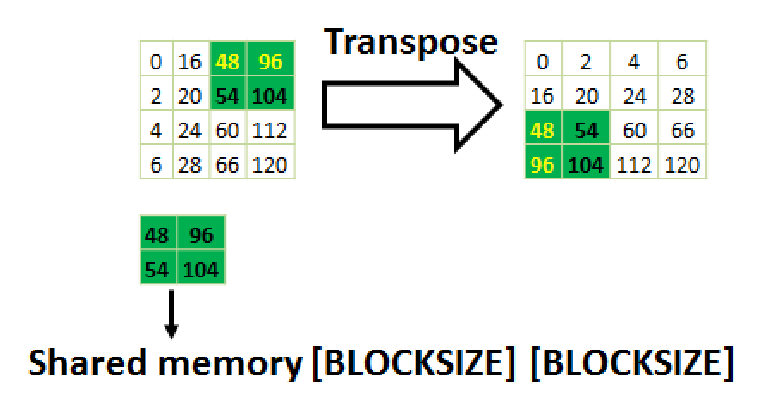
\includegraphics[width=\linewidth]{figs/nn_naive_crop.pdf}
  \caption{Naive Implementation of Matrix Transpose }
  \label{fig:naive}
\end{figure}

\begin{figure}[h]
  \centering
  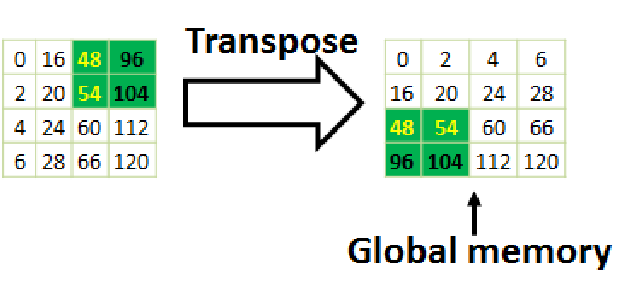
\includegraphics[width=0.9\linewidth]{figs/nn_optim_crop.pdf}
  \caption{Optimized Implementation of Matrix Transpose }
  \label{fig:optim}
\end{figure}

However, changing the reading pattern from a shared memory from 
row wise(Figure~\ref{fig:naive}) to column wise(Figure~\ref{fig:optim}), we need to make sure there 
aren’t any shared memory bank conflicts.

\vspace{0.1in}
\item \textbf{Elimination Of shared memory bank conflicts:}
SM bank conflicts occur when two or more threads in the same warp try to access the same memory bank. 
Let’s analyze the thread mapping to shared memory banks for this situation. Here in our implementation, 
we use a BLOCKSIZE of  16. Each (Tx, Ty) map to (Tx * 16 + Ty) \% 32  bank of an SM. (Tx, Ty) for (0, 0) \& (2, 0) 
\textit{(have global thread indices of 0 and 2 respectively, so belong to the same warp)} map to bank 0. 
So, we have a 2-way bank conflict introduced with the change in access pattern to SM. However, 
it is eliminated by making the (Tx * 16 + Ty) not a multiple of 32. 
Shared memory [BLOCKSIZE] [BLOCKSIZE + 1] was used to tackle this problem. 
Increasing the row width by 1 makes each mapping offset by 1 bank position.


\vspace{0.1in}
\item  \textbf{Use Extern To Declare Shared Memory:}
Hard coding the shared memory size tends to make it an inherent occupancy constraint 
though in practice it can be avoided. Instead, we can make it as extern, 
determine the size during runtime and pass it in kernel launch. Let’s analyze the 
RowScan kernel configuration to brief this situation.  

Kernel configuration: (w, h – width \& height of downscaled Image)
\begin{itemize}
    \item Threads per block = smallestpower2(w): Constraint from RowScan algorithm
    \item Blocks = h
    \item shared memory of 2 * (width of image + 1) (factor 2: One for integral sum \& other for square Integral sum).
\end{itemize}
At downscale of 256 X 256 image size (from source of 1024 X 1024 pixels), we launch a 1 dimensional 
grid of 256 blocks with 256 Threads Per Block (TPB). For this configuration, 6 blocks can be alive, 
giving a 100\% occupancy (1536 threads). Hardcoding the shared memory to that of max case 
of 1024 TPB (8kB SM)  decreases it to 5 blocks giving 84\% occupancy only. 

\end{itemize}


\subsection{Optimizations for Scan Window Processing}\label{sec:haar_optim}
\begin{itemize}

\item \textbf{Using Shared Memory:}
Information about the classifiers as mentioned in Section
\ref{sec:haar} are common to all the scan windows. Hence the first optimization 
is to bring the data related to classifiers. But since there are 2913 classifiers 
for the entire face detection process, it requires 209.836kB of storage for the data. 
But a maximum of 48kB shared memory is available. Hence we split the scan window processing 
into multiple kernels with n stages in each kernel that correspond to around 320 Haar classifiers. 
This requires 12 kernels with around 19kB of shared memory each.
Using Pinned Host Memory: When allocating memory on CPU for the data that needs to be transferred 
to GPU, there are two types of memory to choose from: \emph{Pinned} and \emph{Non-Pinned}. 
Pinned memory is not swapped out from the memory by the OS for any reason and hence provides 
improved transfer speeds. CUDA provides \emph{cudaMallocHost} API that can be used instead of 
usual \emph{malloc} to achieve this.

\vspace{0.1in}
\item \textbf{Using Fast Math:}
Our algorithm makes use of calculating standard deviation which is the square 
root of variance. If we make use of \emph{-use\_fast\_math} flag while compiling using \emph{nvcc}, 
we explicitly instruct GPU to use its Special Functional Unit to calculate square root. This provides 
lesser precision but at a greater speed. 

\vspace{0.1in}
\item \textbf{Not using restriction on maximum registers per thread:}
In our baseline implementation, we had 
restricted maximum register count per thread to 20 to increase occupancy. But scanning window 
kernel requires 28 registers. Because of the restriction there was spilling of registers that 
increased the execution time. Hence we removed the imposition and observed decreased execution 
time even though occupancy decreased. This showed occupancy is not always a measure of performance.

\vspace{0.1in}
\item \textbf{Using block divergence:}
In the baseline implementation, each thread continued execution up to 25 stages 
even if the scan window failed any previous stage. Rejecting a thread as early as possible leads to thread 
divergence that leads to under-utilization as in Figure~\ref{fig:tdiv}. But if all the threads in a block 
are rejected, block divergence occurs and the entire block will not be launched at all thus increasing 
performance as in Figure~\ref{fig:bdiv}. Since each kernel can consist of multiple stages, we reject a 
scan window at kernel-level granularity. Images that have one or two faces have only few scan windows that 
have face. Using this optimization, we have made the common case faster. Hence according to 
\emph{Amdahl’s law} we observe huge increase in performance. 

\end{itemize}
\begin{figure}[h]
  \centering 
  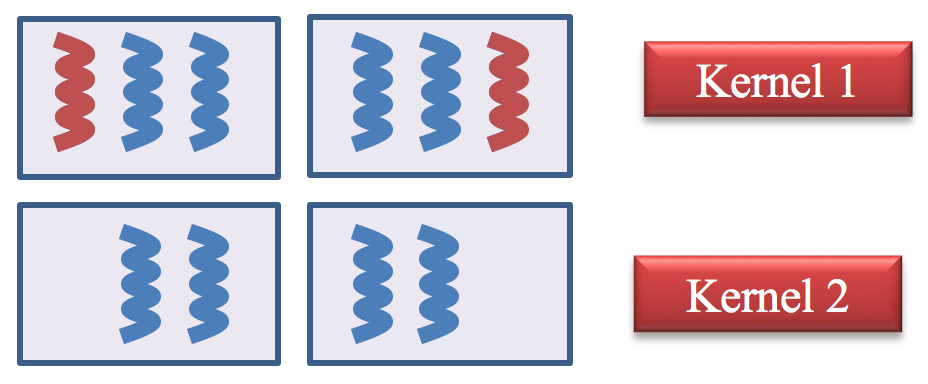
\includegraphics[width=\linewidth]{figs/thread_div.png}
  \caption{Example of Thread Divergence \textnormal{\small }  }
  \label{fig:tdiv}
\end{figure}


\begin{figure}[h]
  \centering 
  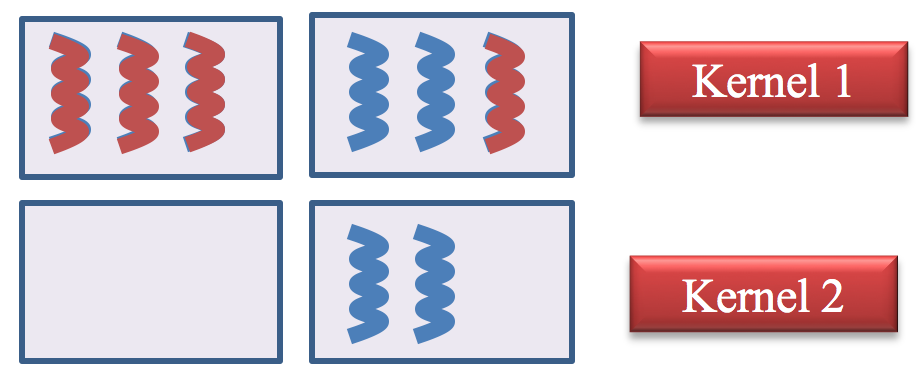
\includegraphics[width=\linewidth]{figs/block_div.png}
  \caption{Example of Block Divergence \textnormal{\small }  }
  \label{fig:bdiv}
\end{figure}


